\documentclass[aspectratio=169]{beamer}
\usetheme{Boadilla}
\beamertemplatetransparentcoveredhigh
\usepackage[portuges]{babel}
\usepackage[utf8]{inputenc}
\usepackage[alf]{abntex2cite}	
\usepackage[portuguese, linesnumbered, vlined, titlenumbered, ruled]{algorithm2e}
%\usepackage{beamerthemesplit}
\usepackage{multirow}
\usepackage{scalefnt}
\usepackage{amssymb}
\usepackage{mathtools}
\usepackage{calrsfs}
% \usepackage{tikz}
% \usetikzlibrary{matrix,backgrounds,matrix,positioning,arrows}
% \usetikzlibrary{patterns,arrows,decorations.pathreplacing}
% The Beamer class comes with a number of default slide themes
% which change the colors and layouts of slides. Below this is a list
% of all the themes, uncomment each in turn to see what they look like.

%\usetheme{default}
%\usetheme{AnnArbor}
%\usetheme{Antibes}
%\usetheme{Bergen}
%\usetheme{Berkeley}
%\usetheme{Berlin}
%\usetheme{Boadilla}
%\usetheme{CambridgeUS}
%\usetheme{Copenhagen}
%\usetheme{Darmstadt}
%\usetheme{Dresden}
%\usetheme{Frankfurt}
%\usetheme{Goettingen}
%\usetheme{Hannover}
%\usetheme{Ilmenau}
%\usetheme{JuanLesPins}
%\usetheme{Luebeck}
%\usetheme{Madrid}
%\usetheme{Malmoe}
%\usetheme{Marburg}
%\usetheme{Montpellier}
%\usetheme{PaloAlto}
%\usetheme{Pittsburgh}
%\usetheme{Rochester}
%\usetheme{Singapore}
%\usetheme{Szeged}
%\usetheme{Warsaw}

% As well as themes, the Beamer class has a number of color themes
% for any slide theme. Uncomment each of these in turn to see how it
% changes the colors of your current slide theme.

%\usecolortheme{albatross}
%\usecolortheme{beaver}
%\usecolortheme{beetle}
%\usecolortheme{crane}
%\usecolortheme{dolphin}
%\usecolortheme{dove}
%\usecolortheme{fly}
%\usecolortheme{lily}
%\usecolortheme{orchid}
%\usecolortheme{rose}
%\usecolortheme{seagull}
%\usecolortheme{seahorse}
%\usecolortheme{whale}
%\usecolortheme{wolverine}

%\setbeamertemplate{footline} % To remove the footer line in all slides uncomment this line
%\setbeamertemplate{footline}[page number] % To replace the footer line in all slides with a simple slide count uncomment this line

%\setbeamertemplate{navigation symbols}{} % To remove the navigation symbols from the bottom of all slides uncomment this line


\usepackage{graphicx} % Allows including images
%\usepackage{booktabs} % Allows the use of \toprule, \midrule and \bottomrule in tables

%----------------------------------------------------------------------------------------
%	TITLE PAGE
%----------------------------------------------------------------------------------------

\title[Tabelas Hash]{Algoritmo e Estrutura de Dados III}
\subtitle{Tabelas Hash}
\author[Frederico Santos de Oliveira]{prof. Frederico Santos de Oliveira}
\institute[UFMT]{Universidade Federal de Mato Grosso\\ Instituto de Engenharia}
\date{}

\AtBeginSection[]
{
	\begin{frame}
	\frametitle{Table of Contents}
	\tableofcontents[currentsection]
\end{frame}
}

\begin{document}

%------------------------------------------------
\begin{frame}
\titlepage % Print the title page as the first slide

\begin{figure}[!h]
  \centering
  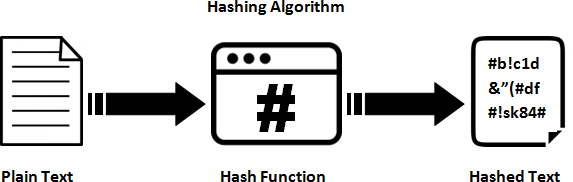
\includegraphics[width=150pt]{imagens/introducao.png}
  \label{fig_introducao}
\end{figure}
\end{frame}

%------------------------------------------------

\begin{frame}
\frametitle{Roteiro} % Table of contents slide, comment this block out to remove it
\tableofcontents % Throughout your presentation, if you choose to use \section{} and \subsection{} commands, these will automatically be printed on this slide as an overview of your presentation
\end{frame}

%----------------------------------------------------------------------------------------
%	PRESENTATION SLIDES
%----------------------------------------------------------------------------------------

%------------------------------------------------
\section{Objetivos}

\begin{frame}
\frametitle{Objetivos}

Esta aula tem como objetivos:

\begin{enumerate}
\item Formalizar a definição de Tabelas Hash,
\item Apresentar os conceitos de Função Hash, Hashing Universal e tratamento de colisões. 
\end{enumerate}
\end{frame}

%------------------------------------------------
\section{Motivação} % Sections can be created in order to organize your presentation into discrete blocks, all sections and subsections are automatically printed in the table of contents as an overview of the talk
%------------------------------------------------

\begin{frame}
\frametitle{Motivação}
\begin{itemize}
 \item Os métodos de pesquisa vistos até agora buscam informações armazenadas com base na comparação de suas chaves.
 \item Esses métodos utilizam listas ou árvores para organizar as informações.
\begin{itemize}
\item Os algoritmos mais eficientes de busca, mostrados até o momento, demandam esforço computacional $O(\log n)$. 
\end{itemize}
 \item Porém, em nenhuma dessas estruturas se obtém o acesso direto a alguma informação, a partir do conhecimento de sua chave. 
\end{itemize}
\end{frame}

\begin{frame}
\frametitle{Aplicações}
\begin{itemize}
 \item Suas aplicações incluem banco de dados, implementações das tabelas de símbolos dos compiladores, na programação de jogos para acessar rapidamente a posição para qual o personagem irá se mover e na implementação de um dicionário.
 \item Em redes de computadores, NAT, {\it Network Address Translation}, também conhecido como masquerading, é uma técnica que consiste em reescrever os endereços IP utilizando-se de uma tabela hash.
\end{itemize}
\end{frame}


%------------------------------------------------
\section{Introdução} % Sections can be created in order to organize your presentation into discrete blocks, all sections and subsections are automatically printed in the table of contents as an overview of the talk
%------------------------------------------------

\begin{frame}
\frametitle{Introdução}
\begin{itemize}
 \item Uma Tabela Hash, também conhecida como tabela de dispersão ou tabela de espalhamento, é uma estrutura de dados especial, que associa chaves e valores. 
 \item Seu objetivo é a partir de uma chave simples, fazer uma busca rápida e obter o valor desejado. 
\end{itemize}
\end{frame}

\begin{frame}
\frametitle{Introdução}
\begin{itemize}
 \item A Tabela Hash leva em conta o valor absoluto de cada chave, interpretado como um valor numérico. 
 \item Através da aplicação de uma função conveniente, a chave é transformada em um endereço de uma tabela 
\end{itemize}
\begin{figure}[!h]
  \centering
  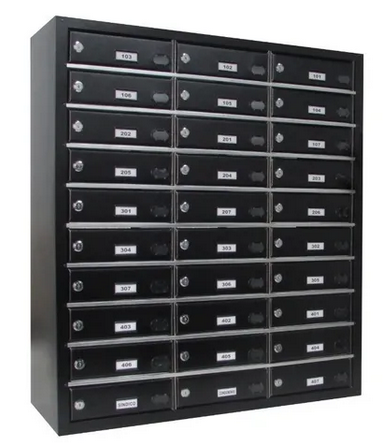
\includegraphics[width=120pt]{imagens/correspondencia.png}
  \label{fig_escaninho}
\end{figure}
\end{frame}

\section{Definição}

\begin{frame}{Introdução}{Princípio de Funcionamento}
\begin{itemize}
 \item Suponha que existam $n$ elementos a serem armazenados em uma tabela $T$, sequencial e de tamanho $m$. 
 \item As posições da tabela se situam no intervalo $[0, m-1]$. 
 \item Isto é, a tabela é particionada em $m$ compartimentos, cada uma corresponde a um endereço, podendo armazenar $m$ elementos.
 \item A forma mais simples de implementar uma {\bf tabela hash} é utilizando {\bf endereçamento direto}.
\end{itemize}
\end{frame}

%\subsection{Endereçamento Direto}

\begin{frame}{Endereçamento Direto}
\begin{itemize}
 \item Cada elemento é identificado por uma chave em $\mathbb{N}$;
 \item Quando o universo de chaves $U = {0, 1, . . . , m - 1}$ é pequeno, a tabela pode ser implementada diretamente como um vetor.
 \item Cada posição representa uma chave de $U$ e armazena um elemento $x$ ou um ponteiro para $x$. 
\end{itemize}
\begin{figure}[!h]
  \centering
  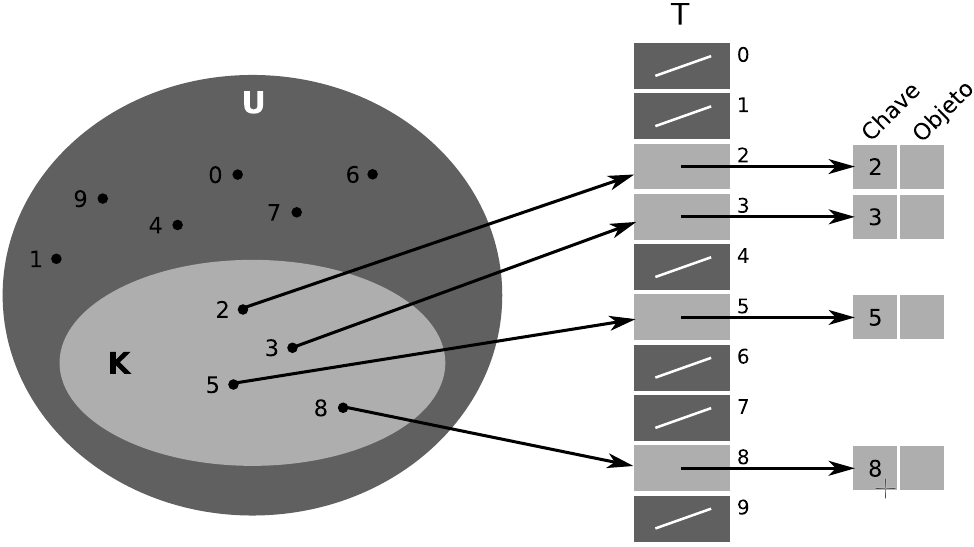
\includegraphics[width=200pt]{imagens/tabela_enderecamento_direto.png}
  \label{fig_tabela_enderecamento_direto}
  \caption{Endereçamento direto. Fonte: \citeonline{Cormen2012}.}
\end{figure}
\end{frame}


\begin{frame}{Endereçamento Direto}{Operações}
As operações disponíveis em Tabelas Hash são:
\begin{itemize}
 \item Inserir-Endereçamento-Direto($T$ , $x$): inserir elemento $x$ na tabela hash $T$;
 \item Remover-Endereçamento-Direto($T$ , $x$): remover elemento $x$ da tabela hash $T$;
 \item Buscar-Endereçamento-Direto($T$ , $k$): retornar elemento com chave $k$ na tabela hash $T$, quando $k \in T$.
\end{itemize}
\end{frame}

\begin{frame}{Endereçamento Direto}{Operações}
 \scalebox{0.9}{
  \begin{algorithm}[H]
  \caption{Inserir-Endereçamento-Direto} 
  \label{Enderecamento-direto-inserir}
  \Entrada{Tabela Hash $T$, Elemento $x$}
  \Inicio{
    $T [key [x]] \leftarrow x$\\
  }
  \end{algorithm}
 }

 \scalebox{0.9}{
  \begin{algorithm}[H]
  \caption{Remover-Endereçamento-Direto} 
  \label{Enderecamento-direto-remover}
  \Entrada{Tabela Hash $T$, Elemento $x$}
  \Inicio{
    $T [key [x]] \leftarrow NULL$\\
  }
  \end{algorithm}
  }
  \scalebox{0.9}{
  \begin{algorithm}[H]
  \caption{Buscar-Endereçamento-Direto} 
  \label{Enderecamento-direto-buscar}
  \Entrada{Tabela Hash $T$, Chave $k$}
  \Inicio{
    \Retorna $T [ k ]$\\
  }
  \end{algorithm}
  }

\tiny{Adaptado de \citeonline{Cormen2012}.}
\end{frame}

\begin{frame}{Endereçamento Direto}{Operações}
\begin{figure}[!h]
  \centering
  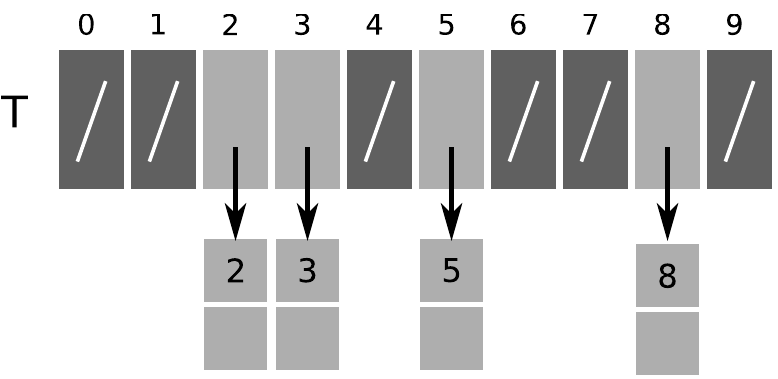
\includegraphics[width=200pt]{imagens/exemplo_tabela_enderecamento_direto.png}
  \label{fig_exemplo_tabela_enderecamento_direto}
  \caption{Endereçamento direto. Fonte: \citeonline{Cormen2012}.}  
\end{figure}
\end{frame}

\begin{frame}{Endereçamento Direto}{Análise}
\begin{itemize}
\item As operações possuem complexidade temporal $O(1)$ (constante) no pior caso.
\item No entanto, se o universo de chaves for muito grande ou esparso, torna-se inviável sua utilização.
\item A solução é utilizar uma função hash $h$ para mapear um elemento $x$ à sua chave $k=h(x)$.
\end{itemize}
\end{frame}

%%------------------------------------------------

%\subsection{Tabelas Hash}

\begin{frame}{Tabelas Hash}
\begin{itemize}
 \item A tabela é implementada como um vetor de $m$ posições em que cada posição armazena um subconjunto de $U$.
\end{itemize}
\begin{figure}[!h]
  \centering
  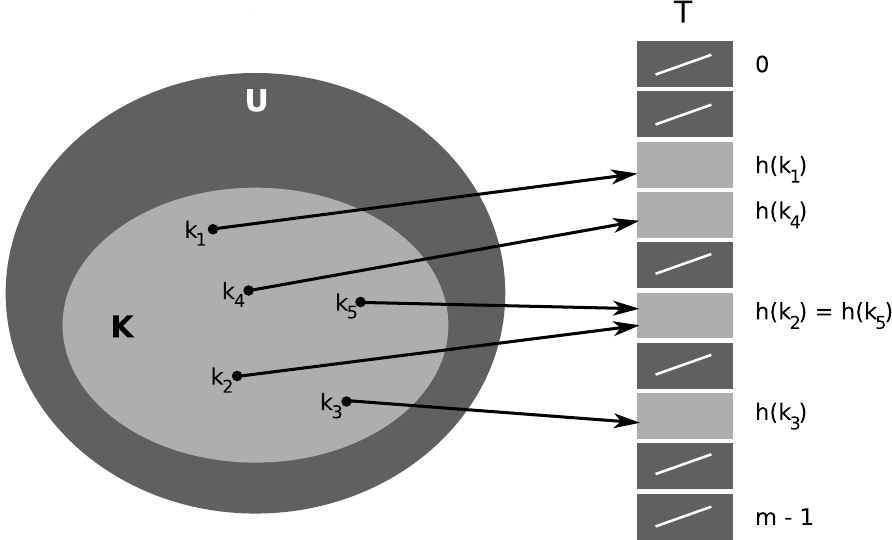
\includegraphics[width=200pt]{imagens/tabela_hash.png}
  \label{fig_tabela_hash}
  \caption{Função hash. Fonte: \citeonline{Cormen2012}.}
\end{figure}
\end{frame}

\begin{frame}{Tabelas Hash}{Vantagens x Desvantagens}
\begin{block}{Vantagem}
Se $K$ é o conjunto das chaves armazenadas, a tabela requer espaço $\Theta(|K|)$ ao invés de $\Theta(|U|)$.
\end{block}
\begin{block}{Desvantagens}
{\color{red} Colisão}: duas chaves podem ser mapeadas para a mesma posição!
A busca na tabela requer O(1) no caso médio, mas O(n) no pior caso.
\end{block}
\end{frame}

\begin{frame}{Tabelas Hash}{Possíveis Problemas}
\begin{block}{Problema}
O número de colisões não pode ser muito grande.
\end{block}
\begin{itemize}
 \item Esse número depende de como a função de hash $h$ espalha os elementos.
 \item {\color{red} Solução}: escolher uma função h determinística, mas com saída aparentemente aleatória.
\end{itemize}
\end{frame}


\section{Projeto de Funções Hash}


\begin{frame}{Projeto de Funções Hash}
\begin{block}{Problema}
Funções de hash verdadeiramente aleatórias não podem ser implementadas com tempo constante.
\end{block}
\begin{itemize}
\item Precisamos de uma função que pareça aleatória, ou seja, mapeie um elemento para cada posição com probabilidade próxima de $\frac{1}{m}$. \item Isso depende da distribuição das entradas.
\end{itemize}
\end{frame}

\begin{frame}{Projeto de Funções Hash}
Exemplos:
\begin{itemize}
 \item Se as entradas $k$ são valores reais uniformemente distribuídos no intervalo $[0, 1)$, podemos usar $h(k) = \lfloor km \rfloor$;
 \item Se as entradas são identificadores de um programa, $h$ deve diminuir a probabilidade de elementos parecidos como ``pt'' e ``pts'' colidirem.
\end{itemize}
\end{frame}

%\subsection{Método da Divisão}

\begin{frame}{Projeto de Funções Hash}{Método da Divisão}
\begin{block}{Método da Divisão}
A função $h$ é definida como $h(k) = k \mod m$.
\end{block}
A qualidade depende da escolha de $m$:
 \begin{itemize}
 \item Se $m = 2^p$, a função escolhe os bits menos significativos de $k$;
 \item Se $m$ é um número primo não muito próximo de uma potência de $2$, $h$ considera mais bits de $k$.
 \end{itemize}
\end{frame}

\begin{frame}{Projeto de Funções Hash}{Método da Divisão}
Exemplo
\begin{itemize}
\item Para armazenar $n = 2000$ elementos em uma tabela de hash , onde uma busca sem sucesso pode visitar até 3 elementos, $m$ deve ser primo e próximo de $\frac{2000}{3}$. 
\pause
\begin{itemize}
\item Um bom valor para $m$ é 701.
\item Um valor ruim é 500.
\end{itemize}
\end{itemize}
\end{frame}

\begin{frame}{Projeto de Funções Hash}{Método da Divisão}
\begin{itemize}
 \item Determine os resultados de $h(k) = k \mod m$, utilizando os dois valores de $m=500$ e $m=701$, para as chaves
\begin{equation}
k = \{501,601,1000,1500,1101,1501\} \nonumber
\end{equation}  
Utilizando a função hash
\begin{equation}
h(k) = k \mod m \nonumber
\end{equation}
\end{itemize}
\end{frame}



\begin{frame}{Percurso}{Busca em Profundidade}
\centering{$h(k) = k \mod m$}
\begin{columns}
\begin{column}{0.5\textwidth}
  \begin{center}
  $m = 701$.
  \begin{eqnarray}
  h(501) &=& 501 \nonumber\\
  h(601) &=& 601 \nonumber\\
  h(1000) &=& 299 \nonumber\\
  h(1101) &=& 400 \nonumber\\
  h(1500) &=& 98 \nonumber\\
  h(1501) &=& 99 \nonumber
  \end{eqnarray}
  \end{center}
\end{column}
\begin{column}{0.5\textwidth}  
  \begin{center}
  
  $m = 500$.
  \begin{eqnarray}
  h(501) &=& 1 \nonumber\\
  h(601) &=& 101 \nonumber\\
  h(1000) &=&  0 \nonumber\\
  h(1101) &=& 101 \nonumber\\
  h(1500) &=& 0 \nonumber\\
  h(1501) &=& 1 \nonumber
  \end{eqnarray}
  \end{center}
\end{column}
\end{columns}
\end{frame}

%\subsection{Método da Multiplicação}


\begin{frame}{Projeto de Funções Hash}{Método da Multiplicação}
\begin{block}{Método da Multiplicação}
A função $h$ é definida como $h(k) = \lfloor m(kc \mod 1) \rfloor $.
\end{block}
\begin{block}{Função h}
$k c \mod 1$ significa a parte fracionária de $kc$, que é $kc - \lfloor kc \rfloor$. Portanto, $h(k) = \lfloor m (kc - \lfloor kc \rfloor ) \rfloor $.
\end{block}
 \begin{itemize}
 \item Neste caso, o valor de $m$ não é crítico, mas a escolha de $c$ depende das características da entrada.
 \item Mas, a escolha da constante $c$ é importante. 
 \end{itemize}
\end{frame}

\begin{frame}{Projeto de Funções Hash}{Método da Multiplicação}
Exemplo:
 \begin{itemize}
 \item Considere os valores $m = 1000$ e $c = 0,5$.
 \item Determine os resultados de h(k) para
\begin{equation}
k = \{1100,1101,1102,1103,1104,1105\} \nonumber
\end{equation}  
\end{itemize}
\end{frame}

\begin{frame}{Projeto de Funções Hash}{Método da Multiplicação}
$m = 1000$ e $c = 0,5$.
\begin{eqnarray}
h(1100) &=& 0 \nonumber\\
h(1101) &=& 500 \nonumber\\
h(1102) &=&  0 \nonumber\\
h(1103) &=& 500 \nonumber\\
h(1104) &=& 0 \nonumber\\
h(1105) &=& 500 \nonumber\\
h(1106) &=& 0 \nonumber\\
h(1107) &=& 500 \nonumber
\end{eqnarray}
\pause {\color{red}Colisão!}
\end{frame}

\begin{frame}{Projeto de Funções Hash}{Método da Multiplicação}
\begin{itemize}
\item Alguns valores de c são melhores do que outros.
\item Em especial, $c = \frac{\sqrt{5} - 1}{2} \approx 0,6180339887...$. Ou seja, a razão áurea!
\item \citeonline{Knuth1997} mostrou por meio de experimentos que o uso da razão áurea apresenta bons resultados.
\end{itemize}
\end{frame}


%\subsection{Mapeamento Universal}

\begin{frame}{Projeto de Funções Hash}{Mapeamento Universal}
\begin{block}{Problema}
Heurísticas são determinísticas e podem ser manipuladas de forma indesejada. Um adversário pode escolher as chaves de entrada para que todas colidam.
\end{block}
%{\color{red} Solução}: no início da execução, escolher aleatoriamente uma função de hash de uma classe $\mathcal{H}$ de funções determinísticas.
\begin{itemize}
\item Uma estratégia que tenta minimizar o problema de colisões é o hashing universal.
\item A idéia é escolher aleatóriamente (em tempo de execução) uma função hash a partir de um conjunto de funções cuidadosamente desenhado.
\end{itemize}

\end{frame}

\begin{frame}{Projeto de Funções Hash}{Mapeamento Universal}
\begin{block}{Definição}
Uma classe $\mathcal{H}$ de funções de hash é universal se o número de funções $h \in \mathcal{H}$ em que $h(k_i) = h(k_j)$ é $\frac{|\mathcal{H}|}{m}$.
\end{block}
\end{frame}

\begin{frame}{Mapeamento Universal}{Análise}
\begin{itemize}
 \item A colisão entre duas chaves $k_i$ e $k_j$ ocorre com probabilidade  $\frac{1}{m}$, a mesma probabilidade de colisão se $h(k_i)$ e $h(k_j)$ fossem selecionados aleatoriamente em $\mathcal{H}$.
 \item O limite superior para o número esperado de colisões para cada chave $k$, baseando-se na escolha da função de hash é:
 \begin{equation}
  \sum_{i \in T, i \neq k} \frac{1}{m}. \nonumber
 \end{equation}
 \item Se $k \notin T$, a lista $n_h(k)$ tem tamanho esperado $\frac{n}{m} = \alpha$;
 \item Se $k \in T$, a lista $n_h(k)$ tem tamanho esperado $1 + \frac{n-1}{m} < 1+ \alpha$.
\end{itemize}
\end{frame}

\begin{frame}{Mapeamento Universal}{Análise}
\begin{block}{Teorema}
Com mapeamento universal e encadeamento, o tamanho esperado de cada lista $n_i$ é no máximo $1 + \alpha$.
\end{block}
\begin{block}{Corolário}
Com mapeamento universal e encadeamento, uma tabela com $m$ posições realiza qualquer sequência de $n$ operações contendo $O(m)$ inserções em tempo esperado $\Theta(n)$.
\end{block}
{\color{red}Complexidade}: as operações tomam tempo constante em média.
\end{frame}

\begin{frame}{Mapeamento Universal}{Projeto}
Seja $p$ um número primo tal que $p > |U|$. Denota-se por $\mathbb{Z}_p = {0, 1, . . . , p - 1}$ e $\mathbb{Z}_p^{*} = \mathbb{Z}_p - {0}$.
\begin{block}{Teorema}
A classe $\mathcal{H}_{p,m}$ de funções ${h_{a,b} : a \in \mathbb{Z}_p^{*} , b \in \mathbb{Z}_p }$ é universal para $h_{a,b} (k) = ((a_k + b) \mod p) \mod m$.
\end{block}
{\color{red}Exemplo}: Se p = 17 e m = 16, temos $h_{3,4} (8) = 5$.
A classe tem $p(p - 1)$ funções distintas. A universalidade segue as propriedades da redução módulo o número primo $p$.%
\end{frame}

\section{Tratamento de Colisões}

\begin{frame}{Tratamento de Colisões}
\begin{block}{Problema}
Como $|U| > m$, a escolha de $h$ apenas minimiza o número de colisões.
\end{block}
\begin{itemize}
 \item {\color{red} Solução}: tratar as colisões restantes de forma algorítmica, aplicando:
 \begin{itemize}
 \item {\bf lista encadeada} ou
 \item {\bf endereçamento aberto}.
 \end{itemize}
\end{itemize}
\end{frame}


%\subsection{Lista Encadeada}

\begin{frame}{Tratamento de Colisão}{Lista Encadeada}
\begin{itemize}
 \item Em uma tabela de hash encadeada, todos os elementos mapeados para uma mesma posição são armazenados em uma lista ligada.
\end{itemize}
\begin{figure}[!h]
  \centering
  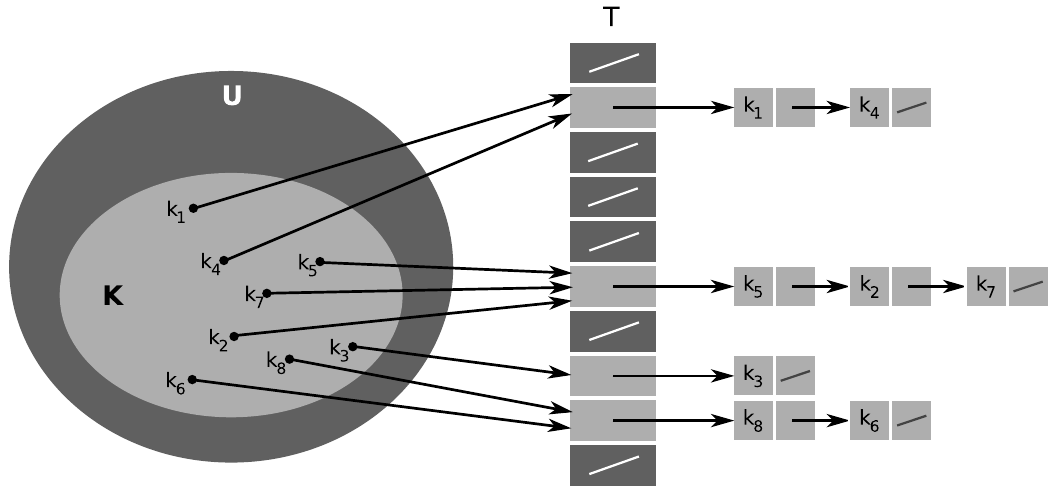
\includegraphics[width=300pt]{imagens/lista_encadeada.png}
  \label{fig_lista_encadeada}
\end{figure}
\end{frame}

%\subsubsection{Exemplo}

\begin{frame}{Tratamento de Colisão}{Lista Encadeada - Exemplo}
\begin{itemize}
 \item Inserção das chaves {5, 28, 19, 15, 20, 33} em uma tabela com 9 posições, utilizando $h(k) = k \mod 9$.
\end{itemize}
\begin{figure}[!h]
  \centering
  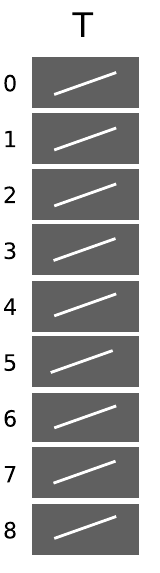
\includegraphics[width=50pt]{imagens/ex_encadeada1.png}
  \label{fig_ex_encadeada1}
\end{figure}
\end{frame}

\begin{frame}{Tratamento de Colisão}{Lista Encadeada - Exemplo}
\begin{itemize}
 \item Inserção da chave 5 para $h(k) = k \mod 9$.
\end{itemize}
\begin{figure}[!h]
  \centering
  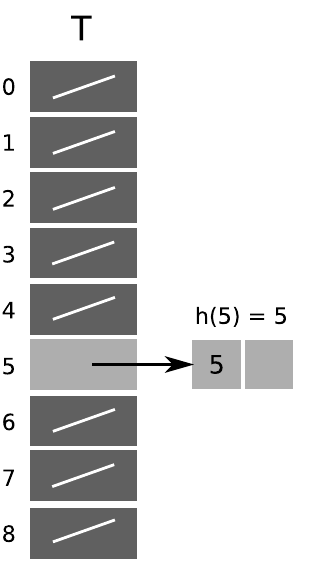
\includegraphics[width=100pt]{imagens/ex_encadeada2.png}
  \label{fig_ex_encadeada2}
\end{figure}
\end{frame}

\begin{frame}{Tratamento de Colisão}{Lista Encadeada - Exemplo}
\begin{itemize}
 \item Inserção da chave 28 para $h(k) = k \mod 9$.
\end{itemize}
\begin{figure}[!h]
  \centering
  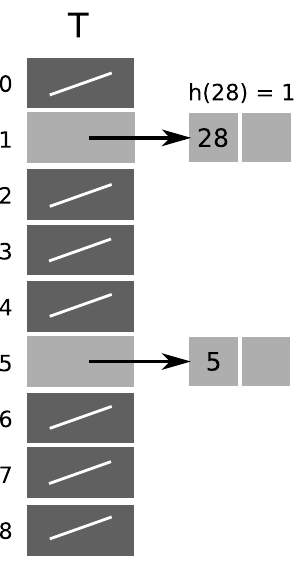
\includegraphics[width=100pt]{imagens/ex_encadeada3.png}
  \label{fig_ex_encadeada3}
\end{figure}
\end{frame}


\begin{frame}{Tratamento de Colisão}{Lista Encadeada - Exemplo}
\begin{itemize}
 \item Inserção da chave 19 para $h(k) = k \mod 9$.
\end{itemize}
\begin{figure}[!h]
  \centering
  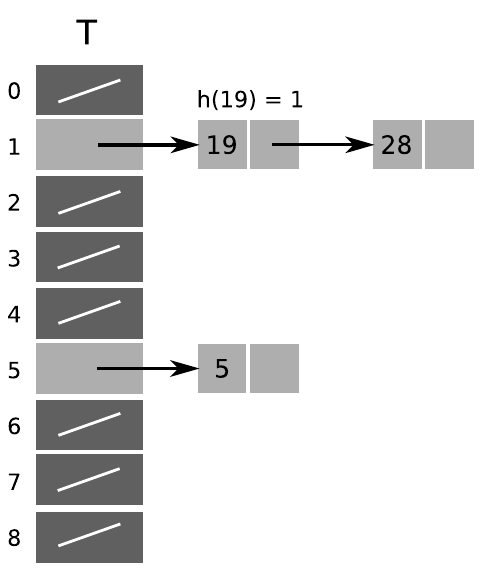
\includegraphics[width=100pt]{imagens/ex_encadeada4.png}
  \label{fig_ex_encadeada4}
\end{figure}
\end{frame}


\begin{frame}{Tratamento de Colisão}{Lista Encadeada - Exemplo}
\begin{itemize}
 \item Inserção da chave 15 para $h(k) = k \mod 9$.
\end{itemize}
\begin{figure}[!h]
  \centering
  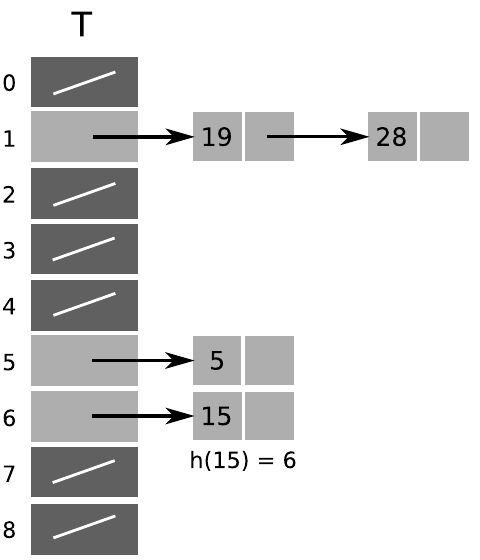
\includegraphics[width=100pt]{imagens/ex_encadeada5.png}
  \label{fig_ex_encadeada5}
\end{figure}
\end{frame}

\begin{frame}{Tratamento de Colisão}{Lista Encadeada - Exemplo}
\begin{itemize}
 \item Inserção da chave 20 para $h(k) = k \mod 9$.
\end{itemize}
\begin{figure}[!h]
  \centering
  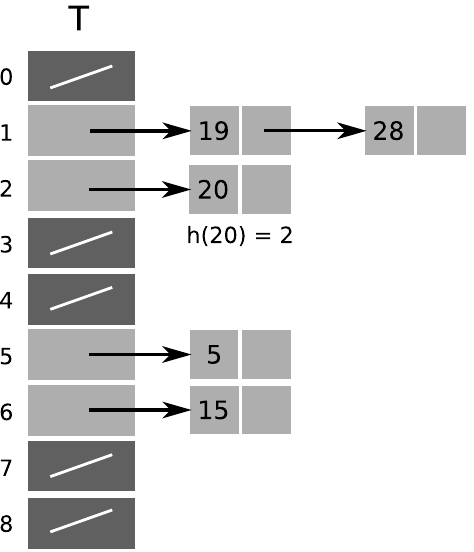
\includegraphics[width=100pt]{imagens/ex_encadeada6.png}
  \label{fig_ex_encadeada6}
\end{figure}
\end{frame}

\begin{frame}{Tratamento de Colisão}{Lista Encadeada - Exemplo}
\begin{itemize}
 \item Inserção da chave 33 para $h(k) = k \mod 9$.
\end{itemize}
\begin{figure}[!h]
  \centering
  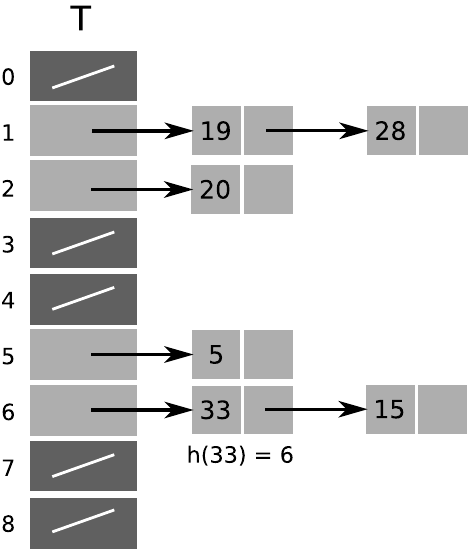
\includegraphics[width=100pt]{imagens/ex_encadeada7.png}
  \label{fig_ex_encadeada7}
\end{figure}
\end{frame}

%\subsubsection{Operações}

\begin{frame}{Lista Encadeada}{Operações}
As operações disponíveis em Tabelas Hash são:
\begin{itemize}
 \item Inserir-Hash-Encadeado($T$ , $x$): inserir elemento $x$ no início da lista $T[ h ( key(x) )]$;
 \item Remover-Hash-Encadeado($T$ , $x$): remover elemento $x$ da lista $T[ h ( key(x) )]$;
 \item Buscar-Hash-Encadeado($T$ , $k$): retornar elemento com chave $k$ na lista $T[ h (k)]$.
\end{itemize}
\end{frame}

\begin{frame}{Lista Encadeada}{Operações}

 \scalebox{0.9}{
  \begin{algorithm}[H]
  \caption{Inserir-Hash-Encadeado} 
  \label{Inserir-Hash-Encadeado}
  \Entrada{Tabela Hash $T$, Elemento $x$}
  \Inicio{
    Inserir $x$ no início da lista $T [ h ( key [x] ) ]$\\
  }
  \end{algorithm}
 }

 \scalebox{0.9}{
  \begin{algorithm}[H]
  \caption{Remover-Hash-Encadeado} 
  \label{Remover-Hash-Encadeado}
  \Entrada{Tabela Hash $T$, Elemento $x$}
  \Inicio{
    Remover $x$ da lista $T [h ( key [x] ) ]$\\
  }
  \end{algorithm}
  }
  \scalebox{0.9}{
  \begin{algorithm}[H]
  \caption{Buscar-Hash-Encadeado} 
  \label{Buscar-Hash-Encadeado}
  \Entrada{Tabela Hash $T$, Chave $k$}
  \Inicio{
    Buscar por um elemento com chave $k$ na lista $T [ h(k) ]$\\
  }
  \end{algorithm}
  }

\tiny{Adaptado de \citeonline{Cormen2012}.}
\end{frame}

\begin{frame}{Lista Encadeada}{Análise}
\begin{itemize}
\item Ao se trabalhar com listas encadeadas, é usual efetuar-se a inserção de uma nova chave $x$ no final da lista correspondente ao endereço $h(x)$.
\item A ideia é que a lista será percorrida de qualquer maneira, para assegurar que $x$ não pertence à mesma.
\item Mas, caso chaves repetidas sejam aceitas, essa condição pode ser relaxada, e a chave inserida no início da lista.
\end{itemize}
\end{frame}

\begin{frame}{Lista Encadeada}{Análise}
\begin{itemize}
 \item Inserção: Complexidade Temporal constante ( $O(1)$ );
 \item Remoção: Complexidade Temporal constante ( $O(1)$ ) utilizando lista duplamente ligada.
 \item Busca sem sucesso: depende do comprimento de $T [h(k)]$;
 \item Busca com sucesso: depende do número de elementos antes de $x$ em $T [h(key [x])]$;
\end{itemize}
\end{frame}

\begin{frame}{Lista Encadeada}{Análise}
No pior caso, todos os elementos são mapeados para a mesma posição e a busca custa $\Theta(n)$ mais o cálculo de $h$.
\begin{block}{Mapeamento uniforme simples}
No caso médio, podemos assumir que um elemento pode ser mapeado para qualquer posição igualmente e que dois elementos são mapeados independentemente:
\begin{equation}
Pr\{h(k_i) = h(k_j )\} = \frac{1}{m}. \nonumber
\end{equation}
\end{block}
\end{frame}

\begin{frame}{Lista Encadeada}{Análise}
\begin{block}{Definição}
Em uma tabela de hash com m posições que armazena n elementos, o fator de carga $\alpha$ é definido como $\frac{n}{m}$.
\end{block}
Seja $n_j$ o comprimento da lista $T [j]$. O valor esperado de $n_j$ é $\alpha$. Assume-se que para calcular $k = h(x)$ necessite de tempo constante $O(1)$.
\end{frame}

\begin{frame}{Lista Encadeada}{Análise}
\begin{itemize}
 \item {\bf Busca Sem Sucesso}: examina-se toda a lista $T [k]$ com tamanho esperado $\alpha$. A complexidade é $O(1 + \alpha)$.
 \item {\bf Busca Com Sucesso}: examinam-se os elementos anteriores a $x$ e o próprio $x$. Na média, examinam-se
\end{itemize}
 \begin{equation}
  1+ \frac{1}{n} \sum^{n}_{i=1} \sum^{n}_{j=i+1} \frac{1}{m} = O (1 + \frac{1}{n} \frac{1}{m} n^2) = O (1 + \alpha). \nonumber
 \end{equation}

\end{frame}


\begin{frame}{Lista Encadeada}{Análise}
\begin{itemize}
 \item Se o número de posições é proporcional ao número de elementos, ou n = O(m), o fator de carga é $\alpha = O(1)$ e a busca toma tempo constante no caso médio;
 \item Todas as operações tomam tempo constante em média.
\end{itemize}
\end{frame}

%\subsection{Endereçamento Aberto}

\begin{frame}{Tratamento de Colisão}{Endereçamento Aberto}
\begin{itemize}
 \item Em uma tabela de hash com endereçamento aberto, todos os elementos são armazenados na tabela propriamente dita. 
 \item O espaço gasto com encadeamento é economizado e a colisão é tratada com a busca de uma nova posição para inserção.
 \item Naturalmente, o fator de carga não pode exceder o valor 1.
\end{itemize}
\begin{figure}[!h]
  \centering
  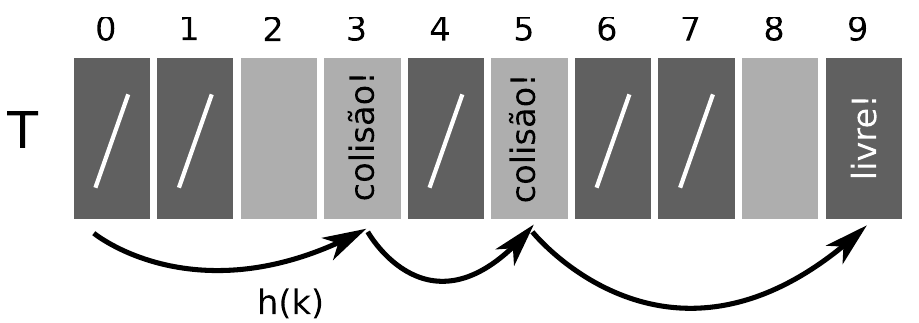
\includegraphics[width=300pt]{imagens/enderecamento_aberto.png}
  \label{fig_enderecamento_aberto}
\end{figure}
\end{frame}

%\subsubsection{Operações}

\begin{frame}{Endereçamento Aberto}{Operações}
Durante a inserção, uma sequência de posições é testada até que uma posição livre seja encontrada. A função de hash é modificada para receber um argumento que armazena o número do teste.
\scalebox{0.85}{  
  \begin{algorithm}[H]
  \caption{Inserir-Hash-Aberto} 
  \label{Inserir-Hash-Aberto}
  \Entrada{Tabela Hash $T$, Elemento $x$}
  \Inicio{
    $i \leftarrow 0$\\
    \Repita {(i=m)} {
      $j \leftarrow h(k,i)$\\
      \Se {(T[j] = NULL)} {
	T[j] $\leftarrow$ k \\
	\Retorna j 
      }
      \Senao {
	$i\leftarrow i + 1$\\ 
      }
    }
    Imprima (``Erro: Overflow'') \\
  }
  \end{algorithm}
}

\tiny{Adaptado de \citeonline{Cormen2012}.}
\end{frame}

\begin{frame}{Endereçamento Aberto}{Operações}
O algoritmo de busca percorre a mesma sequência examinada pelo algoritmo de inserção quando $k$ foi inserido.
\scalebox{0.9}{  
  \begin{algorithm}[H]
  \caption{Buscar-Hash-Aberto} 
  \label{Buscar-Hash-Aberto}
  \Entrada{Tabela Hash $T$, Chave $k$}
  \Inicio{
    $i \leftarrow 0$\\
    \Repita {(T[j]=NULL ou i = m)} {
      $j \leftarrow h(k,i)$\\
      \Se {(T[j] = k)} {
	\Retorna j \\
      }
      \Senao {
	$i\leftarrow i + 1$\\ 
      }
    }
    \Retorna NULL \\
  }
  \end{algorithm}
}

\tiny{Adaptado de \citeonline{Cormen2012}.}
\end{frame}

\begin{frame}{Endereçamento Aberto}{Operações}
\begin{itemize}
\item A {\bf remoção} de elementos é difícil. 
\item Pode-se utilizar um valor especial para marcar elementos removidos.
\item Mas o custo da busca deixa de depender do fator de carga.
\end{itemize}
\end{frame}

%\subsubsection{Busca Linear}

\begin{frame}{Endereçamento Aberto}{Busca Linear}
A função de hash deve produzir como sequência de teste uma permutação de ${0, 1, . . . , m - 1}$.
\begin{block}{Busca linear}
Seja $h$ uma função de hash auxiliar. A função $h$ é definida como $h(k, i) = (h' (k) + i) \mod m$.
\end{block}
\end{frame}

\begin{frame}{Busca Linear}{Vantagens x Desvantagens}
\begin{block}{Vantagem}
Fácil implementação.
\end{block}
\begin{block}{Desvantagem}
É suscetível a {\bf agrupamento primário}. Ou seja, são construídas sequências longas de posições ocupadas, o que degrada o desempenho da busca.
\end{block} 
\end{frame}

%\subsubsection{Exemplo}

\begin{frame}{Busca Linear}{Exemplo}
Inserção das chaves $\{10, 22, 31, 4, 15, 28, 59\}$ em uma tabela de tamanho 11 com teste linear e função $h(k, i) = (k + i) \mod 11$.
\begin{figure}[!h]
  \centering
  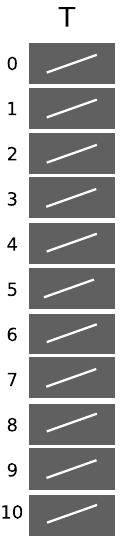
\includegraphics[width=40pt]{imagens/ex_enderecamento_aberto1.png}
  \label{fig_ex_enderecamento_aberto1}
\end{figure}
\end{frame}

\begin{frame}{Busca Linear}{Exemplo}
Inserção da chave 10 para $h(k, i) = (k + i) \mod 11$.
\begin{figure}[!h]
  \centering
  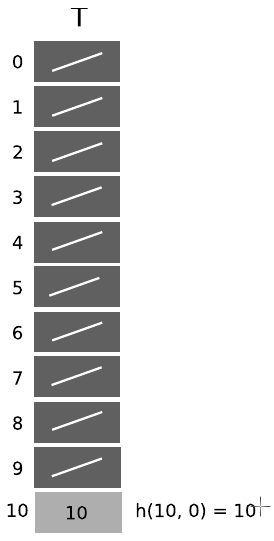
\includegraphics[width=90pt]{imagens/ex_enderecamento_aberto2.png}
  \label{fig_ex_enderecamento_aberto2}
\end{figure}
\end{frame}

\begin{frame}{Busca Linear}{Exemplo}
Inserção da chave 22 para $h(k, i) = (k + i) \mod 11$.
\begin{figure}[!h]
  \centering
  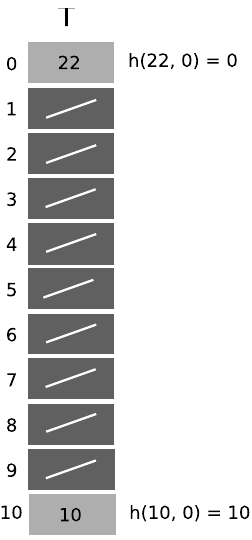
\includegraphics[width=88pt]{imagens/ex_enderecamento_aberto3.png}
  \label{fig_ex_enderecamento_aberto3}
\end{figure}
\end{frame}

\begin{frame}{Busca Linear}{Exemplo}
Inserção da chave 31 para $h(k, i) = (k + i) \mod 11$.
\begin{figure}[!h]
  \centering
  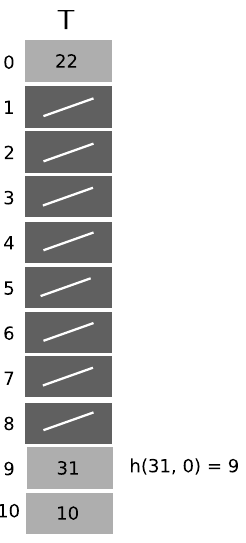
\includegraphics[width=86pt]{imagens/ex_enderecamento_aberto4.png}
  \label{fig_ex_enderecamento_aberto4}
\end{figure}
\end{frame}


\begin{frame}{Busca Linear}{Exemplo}
Inserção da chave 4 para $h(k, i) = (k + i) \mod 11$.
\begin{figure}[!h]
  \centering
  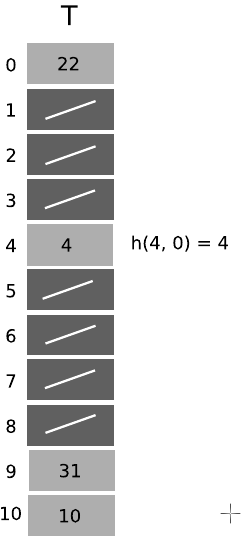
\includegraphics[width=84pt]{imagens/ex_enderecamento_aberto5.png}
  \label{fig_ex_enderecamento_aberto5}
\end{figure}
\end{frame}


\begin{frame}{Busca Linear}{Exemplo}
Inserção da chave 15 para $h(k, i) = (k + i) \mod 11$.
\begin{figure}[!h]
  \centering
  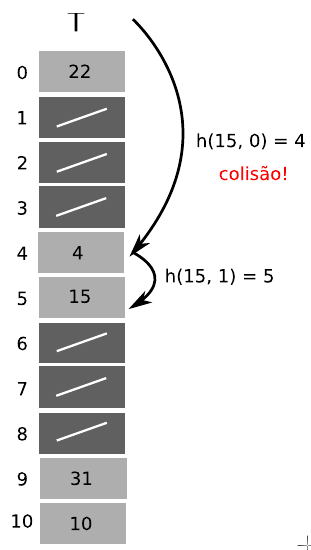
\includegraphics[width=96pt]{imagens/ex_enderecamento_aberto6.png}
  \label{fig_ex_enderecamento_aberto6}
\end{figure}
\end{frame}


\begin{frame}{Busca Linear}{Exemplo}
Inserção da chave 28 para $h(k, i) = (k + i) \mod 11$.
\begin{figure}[!h]
  \centering
  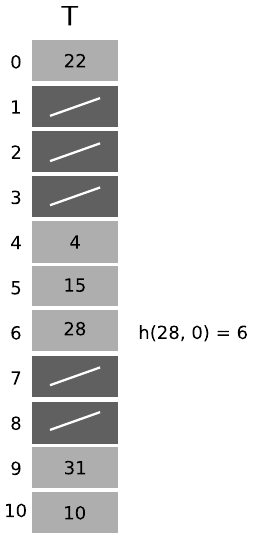
\includegraphics[width=88pt]{imagens/ex_enderecamento_aberto7.png}
  \label{fig_ex_enderecamento_aberto7}
\end{figure}
\end{frame}


\begin{frame}{Busca Linear}{Exemplo}
Inserção da chave 59 para $h(k, i) = (k + i) \mod 11$.
\begin{figure}[!h]
  \centering
  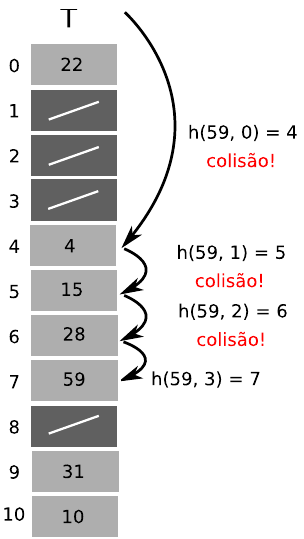
\includegraphics[width=90pt]{imagens/ex_enderecamento_aberto8.png}
  \label{fig_ex_enderecamento_aberto8}
\end{figure}
\end{frame}

%\subsubsection{Busca Quadrática}

\begin{frame}{Endereçamento Aberto}{Busca Quadrática}
\begin{block}{Busca Quadrática}
Seja $h$ uma função de hash auxiliar, $c_1$ e $c_2$ constantes não-nulas. A função $h$ é definida como $h(k, i) = (h' (k) + c_1 i + c_2 i^2 ) \mod m$.
\end{block}
\end{frame}

\begin{frame}{Busca Quadrática}{Vantagens x Desvantagens}
\begin{block}{Vantagem}
É imune a agrupamento primário.
\end{block}
\begin{block}{Desvantagem}
É suscetível a {\bf agrupamento secundário}. Ou seja, as sequuências de teste são idênticas para duas chaves $k_i$ e $k_j$ tais que $h' (k_i ) = h1 (k_j )$.
\end{block} 
\end{frame}


\begin{frame}{Busca Quadrática}{Exemplo}
Inserção das chaves $\{10, 22, 31, 4, 15, 28, 59\}$ em uma tabela de tamanho 11 com teste quadrático e $h(k, i) = (k + i + 3i^2 ) \mod 11$.
\begin{figure}[!h]
  \centering
  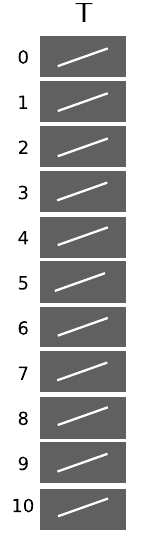
\includegraphics[width=48pt]{imagens/ex_end_aberto_quadratico1.png}
  \label{fig_ex_end_aberto_quadratico1}
\end{figure}
\end{frame}


\begin{frame}{Busca Quadrática}{Exemplo}
Inserção da chave 10 para $h(k, i) = (k + i + 3i^2 ) \mod 11$.
\begin{figure}[!h]
  \centering
  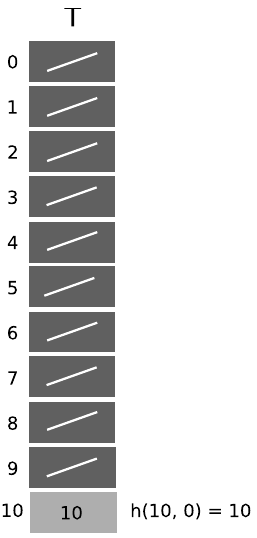
\includegraphics[width=90pt]{imagens/ex_end_aberto_quadratico2.png}
  \label{fig_ex_end_aberto_quadratico2}
\end{figure}
\end{frame}

\begin{frame}{Busca Quadrática}{Exemplo}
Inserção da chave 22 para $h(k, i) = (k + i + 3i^2 ) \mod 11$.
\begin{figure}[!h]
  \centering
  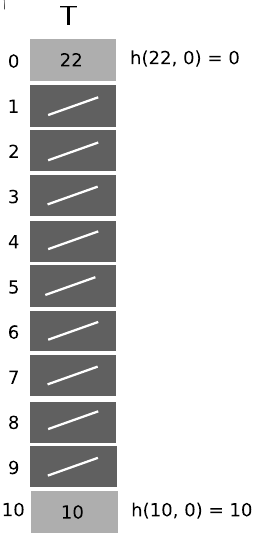
\includegraphics[width=90pt]{imagens/ex_end_aberto_quadratico3.png}
  \label{fig_ex_end_aberto_quadratico3}
\end{figure}
\end{frame}

\begin{frame}{Busca Quadrática}{Exemplo}
Inserção da chave 31 para $h(k, i) = (k + i + 3i^2 ) \mod 11$.
\begin{figure}[!h]
  \centering
  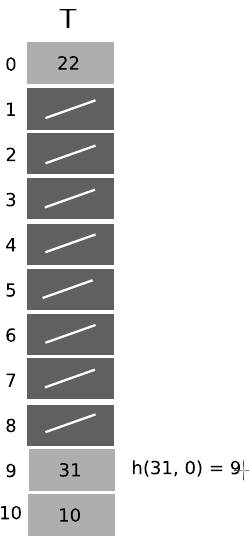
\includegraphics[width=86pt]{imagens/ex_end_aberto_quadratico4.png}
  \label{fig_ex_end_aberto_quadratico4}
\end{figure}
\end{frame}

\begin{frame}{Busca Quadrática}{Exemplo}
Inserção da chave 4 para $h(k, i) = (k + i + 3i^2 ) \mod 11$.
\begin{figure}[!h]
  \centering
  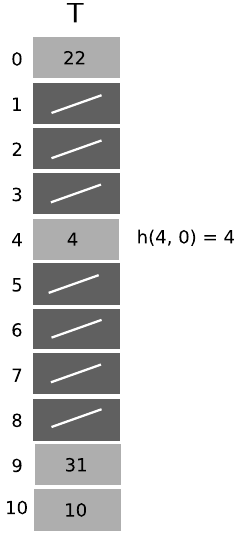
\includegraphics[width=83pt]{imagens/ex_end_aberto_quadratico5.png}
  \label{fig_ex_end_aberto_quadratico5}
\end{figure}
\end{frame}

\begin{frame}{Busca Quadrática}{Exemplo}
Inserção da chave 15 para $h(k, i) = (k + i + 3i^2 ) \mod 11$.
\begin{figure}[!h]
  \centering
  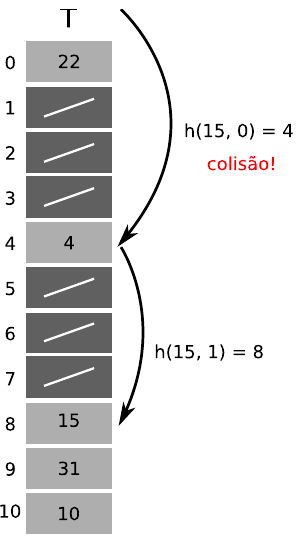
\includegraphics[width=94pt]{imagens/ex_end_aberto_quadratico6.png}
  \label{fig_ex_end_aberto_quadratico6}
\end{figure}
\end{frame}

\begin{frame}{Busca Quadrática}{Exemplo}
Inserção da chave 28 para $h(k, i) = (k + i + 3i^2 ) \mod 11$.
\begin{figure}[!h]
  \centering
  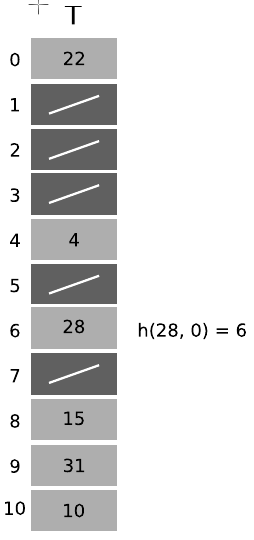
\includegraphics[width=90pt]{imagens/ex_end_aberto_quadratico7.png}
  \label{fig_ex_end_aberto_quadratico7}
\end{figure}
\end{frame}

\begin{frame}{Busca Quadrática}{Exemplo}
Inserção da chave 59 para $h(k, i) = (k + i + 3i^2 ) \mod 11$.
\begin{figure}[!h]
  \centering
  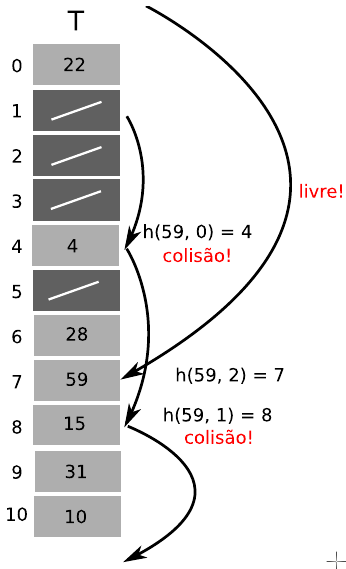
\includegraphics[width=95pt]{imagens/ex_end_aberto_quadratico8.png}
  \label{fig_ex_end_aberto_quadratico8}
\end{figure}
\end{frame}

%\subsubsection{Hash Duplo}

\begin{frame}{Endereçamento Aberto}{Hash Duplo}
\begin{block}{Duplo Mapeamento}
No {\bf hash duplo}, a função $h$ é definida como $h(k, i) = (h_1 (k) + i h_2 (k)) \mod m$, para $1 \leq i \leq m-1$.
\end{block}
\begin{itemize}
\item $h_1$ e $h_2$ são funções de hash auxiliares.
\item O projeto e a implementação são mais difíceis que os métodos apresentados anteriormente.
\item No entanto, não causa agrupamento do tipo produzido pelo teste linear ou pelo teste quadrático, e apresenta
melhor desempenho na média.
\end{itemize}
%É preciso que $h_2 (k)$ e $m$ sejam relativamente primos:
%\begin{itemize}
% \item Escolhe-se $m = 2p$ e $h_2 (k)$ com saída sempre ímpar;
% \item Escolhe-se $m$ primo e $h_2 (k)$ com saída sempre menor que $m$.
%\end{itemize}
\end{frame}

\begin{frame}{Endereçamento Aberto}{Hash Duplo}
\begin{block}{Duplo Mapeamento}
No {\bf hash duplo}, a função $h$ é definida como $h(k, i) = (h_1 (k) + i h_2 (k)) \mod m$, para $1 \leq i \leq m-1$.
\end{block}
\begin{itemize}
\item Para varrer toda a tabela, é necessário que $h_2()$ e $m$ sejam primos entre si, ou seja, o único divisor comum a eles é o número 1.
\item Por exemplo, se $m$ for potência de 2, basta definir $h_2()$ de forma a produzir números ímpares.
\item Ou então, mais simples ainda, basta definir $m$ como um número primo e projetar $h_2()$ de forma que ele sempre retorne um inteiro positivo menor que $m$.
\end{itemize}
\end{frame}

\begin{frame}{Hash Duplo}{Vantagens x Desvantagens}
\begin{block}{Vantages}
\begin{itemize}
\item O mapeamento duplo considera $\Theta(m^2)$ sequências de teste, já que cada par $(h_1 (k), h_2 (k))$ produz uma nova sequência.
\item Teste linear ou quadrático apenas consideram $\Theta(m)$ sequencias.
\end{itemize}
\end{block}
\begin{block}{Desvantagem}
Projeto e implementação mais difícil.
\end{block} 
\end{frame}


%\subsubsection{Exemplo} 

\begin{frame}{Hash Duplo}{Exemplo}
Exemplo:
\begin{itemize}
 \item Sejam $h_1 (k) = k \mod 13$ e $h_2 (k) = 1 + (k \mod 11)$.
 \item Então $h(14, 0) = 1$, $h(14, 1) = 5$ e $h(14, 2) = 9$.
 \begin{itemize}
 \item $h(14, 0) = (h_1 (14) + 0 h_2 (14)) \mod 13 = 1.$
 \item $h(14, 1) = (h_1 (14) + 1 h_2 (14)) \mod 13 = 1 + 1 \times 4  = 5.$
 \item $h(14, 2) = (h_1 (14) + 2 h_2 (14)) \mod 13 = 1 + 2 \times 4 = 9.$
 \end{itemize}
\end{itemize}
\begin{figure}[!h]
  \centering
  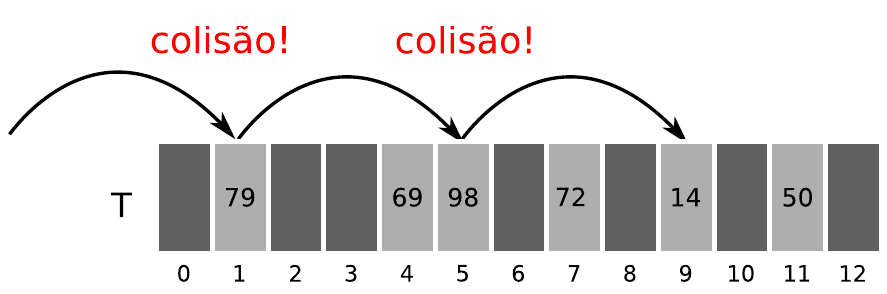
\includegraphics[width=300pt]{imagens/ex_hash_duplo.png}
  \label{fig_ex_hash_duplo}
\end{figure}
\end{frame}

\begin{frame}{Hash Duplo}{Análise}
\begin{itemize}
\item O algoritmo de {\bf pesquisa} (ou busca) percorre a mesma sequência de posições examinada pelo algoritmo de {\bf inserção} quando a chave $k$ foi inserida.
\item Após a {\bf remoção}, a posição não pode ser deixada como uma célula vazia, pois pode interferir nas buscas.
\item A posição deve ser marcada de alguma maneira (com uma variável booleana, por exemplo) para que na busca possa-se saber que havia algo lá.
\end{itemize}
\end{frame}

%
%\begin{frame}{Endereçamento Aberto}{Análise}
%\begin{block}{Mapeamento uniforme}
%No caso médio, podemos assumir que cada chave é mapeada igualmente para cada uma das $m!$ sequências de teste possíveis no conjunto $\{0, 1, . . . , m - 1\}$.
%\end{block} 
%Complexidade
%\begin{itemize}
% \item Busca sem sucesso: proporcional ao número de testes feitos.
% \item O primeiro teste sempre é feito e falha com probabilidade $\alpha$.
% \item O segundo falha com probabilidade $\alpha$ 2 , e assim por diante.
% \item O número de testes é limitado por:
% \begin{equation}
%\sum^{\infty}_{i=1}\alpha^{i-1} = \frac{1}{1-\alpha} = O(1). \nonumber
% \end{equation}
%\end{itemize}
%\end{frame}


%\begin{frame}{Endereçamento Aberto}{Análise}
%Complexidade
%\begin{itemize}
% \item Inserção: consiste em encontrar uma posição desocupada (busca sem sucesso). Logo, a complexidade é O(1) no caso médio.
% \item Busca com sucesso: a busca por uma chave $k$ segue a mesma sequência de teste percorrida na inserção de $k$. Se $k$ foi a $(i + 1)$-ésima chave inserida, o número esperado de testes em uma busca por $k$ é limitado por $\frac{1}{1-i/m} = \frac{m}{m-i}$. A média sobre todas as $n$ chaves é:
%\begin{equation}
%\frac{1}{n} \sum^{n-1}_{i=0} \frac{m}{m-i} \leq \frac{1}{\alpha}/n \frac{1}{1-\alpha} = O(1). \nonumber 
%\end{equation}
%\end{itemize}
%\end{frame}

\begin{frame}{Endereçamento Aberto}{Análise}
Complexidade
\begin{itemize}
 \item Considerando um mapeamento uniforme, o número médio de comparações em uma busca sem sucesso e na inserção é limitado por:

\begin{equation}
\sum^{\inf}_{i=1} \alpha^{i-1} = \frac{1}{1 - \alpha} = O(1). \nonumber
\end{equation}

sendo $\alpha = n/m$ o fator de carga da tabela.

\item O aspecto negativo está relacionado com o pior caso, que é $O(n)$, se a função hash {\bf não} conseguir espalhar os registros de forma razoável pelas entradas da tabela.
\end{itemize}
\end{frame}


\begin{frame}{{Endereçamento Aberto}}{Exercício}
Escreva pseudocódigo para o algoritmo {\bf Remover-Hash-Aberto} e modifique os algoritmos {\bf Inserir-Hash-Aberto} e {\bf Buscar-Hash-Aberto} de forma a levar em conta que elementos removidos da tabela são marcados com o valor especial {\it Deleted}.
\end{frame}

\section{Conclusões}

\begin{frame}{Conclusões}
\begin{itemize}
 \item Considerando um mapeamento uniforme, cada operação toma tempo constante no caso médio. 
 \begin{itemize}
 \item Mas é raro conhecer a distribuição de probabilidade segundo a qual as chaves são obtidas.
 \end{itemize}
\item Na prática, podemos usar heurísticas de fácil implementação para criar uma função hash que provavelmente terá um bom desempenho.
\item Para resolução de colisões, encadeamento é o método mais simples, mas gasta mais espaço.
\item Endereçamento aberto tem implementação mais difícil ou que pode ser suscetível a efeitos de agrupamento.
\end{itemize}
\end{frame}

\begin{frame}{Conclusões}
\begin{itemize}
 \item Vantagens:
 \begin{itemize}
	\item Simplicidade de implementação. 
	\item Considerando K o conjunto de chaves armazenadas, a tabela requer espaço $\Theta(|K|)$ ao invés de $\Theta(|U|)$.
	\item A busca na tabela requer $O(1)$ no caso médio.
 \end{itemize}
 \item Desvantagens:
 \begin{itemize}
\item Colisão: Efeito que acontece quando duas chaves são mapeadas para a mesma posição na tabela. 
\item A busca na tabela requer $O(|k|)$ no pior caso.
 \end{itemize}
\end{itemize}
\end{frame}

%\begin{frame}
%\Huge{\centerline{Dúvidas}}
%\begin{figure}[!h]
%  \centering
%  
\includegraphics[width=200pt]{imagens/duvidas.jpg}
%  \label{fig_fim}
%\end{figure}
%\end{frame}


%------------------------------------------------

\section{Referências bibliográficas}
  \frame{\frametitle{Referências bibliográficas}
    \bibliographystyle{abntex2-alf}
    \bibliography{referencias}
  }

%------------------------------------------------
\section{Material Complementar}
%------------------------------------------------

\begin{frame}{Material Complementar}
   \begin{itemize}
	\item Material Wikibooks
	\begin{itemize}
	 \item \href{https://pt.wikibooks.org/wiki/Algoritmos/Estruturas_de_dados/Tabela_Hash}{https://pt.wikibooks.org/wiki/Algoritmos/Estruturas\_de\_dados/Tabela\_Hash} 
	\end{itemize}		
   \item Animação Método da Divisão - Tratamento de Colisão por lista encadeada.
   \begin{itemize}
   \item \href{https://www.cs.usfca.edu/~galles/visualization/OpenHash.html}{https://www.cs.usfca.edu/~galles/visualization/OpenHash.html}      
   \end{itemize}
   \item Animação Método da Divisão - Tratamento de Colisão por endereçamento aberto.
   \begin{itemize}
   \item \href{https://www.cs.usfca.edu/~galles/visualization/ClosedHash.html}{https://www.cs.usfca.edu/~galles/visualization/ClosedHash.html}   
   \end{itemize}
   \end{itemize}
\end{frame}    


\begin{frame}{Material Complementar}
Youtube
\begin{itemize}
  \item \href{https://www.youtube.com/watch?v=njkANXEMHTY}{Estrutura de Dados Descomplicada - Tabelas Hash}   
  \item \href{https://www.youtube.com/watch?v=M4DGQPF2Oxo}{Prof. Marcos Kutova}   
  \item \href{https://www.youtube.com/watch?v=jQ0r7P8rC1M}{Estruturas de Dados - Conceitos de Tabela Hash (UNIVESP)}    
  \item \href{https://www.youtube.com/watch?v=RmO18m_8ncc}{Estruturas de Dados - Tabela Hash (implementação) (UNIVESP)}      
\end{itemize}	
\end{frame}   

%------------------------------------------------
\begin{frame}
\titlepage % Print the title page as the first slide

\begin{figure}[!h]
  \centering
  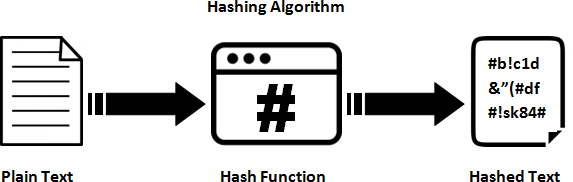
\includegraphics[width=150pt]{imagens/introducao.png}
  \label{fig_introducao}
\end{figure}
\end{frame}
\end{document} 
